\documentclass{scrartcl}

\usepackage[utf8x]{inputenc}
\usepackage{graphicx} % Required for inserting images
\usepackage{booktabs}

\title{Causal Inference for Policy Evaluation}
\subtitle{Assignment 1}
\author{Marco Gortan, Felix Schulz, Benjamin Weggelaar}
\date{March 2025}

\usepackage{xcolor}

\newcommand{\marco}[1]{\textcolor{red}{#1}}
\newcommand{\felix}[1]{\textcolor{cyan}{#1}}
\newcommand{\benji}[1]{\textcolor{green}{#1}}


\begin{document}

\maketitle

\section*{Question 1}

\begin{table}[!h]
\centering
\caption{Share of Age Groups by Treatment Status}
\centering
\begin{tabular}[t]{lr}
\toprule
Treatment Status & $Share \leq 40$\\
\midrule
D=0 & 0.617\\
D=1 & 0.629\\
\bottomrule
\end{tabular}
\end{table}


The differences in the distribution of age across treatment and control groups are relatively small, suggesting that the treatment and control groups are fairly balanced with respect to age. However, the treatment group appears to have a slightly younger composition on average.

\begin{table}[!h]
\centering
\caption{Balance Metrics}
\centering
\begin{tabular}[t]{lrrr}
\toprule
Variable & Standardized Bias & Difference in Means & P-value\\
\midrule
Age & 2.601 & 0.013 & 0.073\\
\bottomrule
\end{tabular}
\end{table}


Here, we test the $H_0$ that the difference in means between the treatment and control group is zero. The p-value of 0.07 is above the conventional 5\% significance level. This suggests that the difference in means is not statistically significant. This indicates that the treatment and control group are balanced with respect to the age variable.

\section*{Question 2}

% \begin{table}[!h]
\tiny
\centering
\caption{Program and Employment: Semiparametric ATE with IPW}
\centering
\begin{tabular}[t]{lrrr}
\toprule
age group & time relative to treatment & effect & se\\
\midrule
above40 & 1 & 0.009 & 0.005\\
above40 & 2 & 0.115 & 0.006\\
above40 & 3 & 0.376 & 0.002\\
above40 & 4 & 0.383 & 0.008\\
above40 & 5 & 0.354 & 0.008\\
\addlinespace
above40 & 6 & 0.328 & 0.004\\
above40 & 7 & 0.293 & 0.001\\
above40 & 8 & 0.257 & 0.002\\
above40 & 9 & 0.221 & 0.000\\
above40 & 10 & 0.197 & 0.008\\
\addlinespace
above40 & 11 & 0.174 & 0.003\\
above40 & 12 & 0.154 & 0.004\\
above40 & 13 & 0.136 & 0.000\\
above40 & 14 & 0.120 & 0.003\\
above40 & 15 & 0.105 & 0.000\\
\addlinespace
above40 & 16 & 0.092 & 0.005\\
above40 & 17 & 0.079 & 0.002\\
above40 & 18 & 0.065 & 0.001\\
above40 & 19 & 0.055 & 0.001\\
above40 & 20 & 0.047 & 0.002\\
\addlinespace
above40 & 21 & 0.041 & 0.001\\
above40 & 22 & 0.035 & 0.004\\
above40 & 23 & 0.008 & 0.000\\
above40 & 24 & 0.004 & 0.000\\
below40 & 1 & 0.009 & 0.001\\
\addlinespace
below40 & 2 & 0.115 & 0.010\\
below40 & 3 & 0.376 & 0.004\\
below40 & 4 & 0.383 & 0.006\\
below40 & 5 & 0.354 & 0.001\\
below40 & 6 & 0.328 & 0.005\\
\addlinespace
below40 & 7 & 0.293 & 0.008\\
below40 & 8 & 0.257 & 0.005\\
below40 & 9 & 0.221 & 0.004\\
below40 & 10 & 0.197 & 0.003\\
below40 & 11 & 0.174 & 0.001\\
\addlinespace
below40 & 12 & 0.154 & 0.008\\
below40 & 13 & 0.136 & 0.002\\
below40 & 14 & 0.120 & 0.002\\
below40 & 15 & 0.105 & 0.001\\
below40 & 16 & 0.092 & 0.001\\
\addlinespace
below40 & 17 & 0.079 & 0.003\\
below40 & 18 & 0.065 & 0.004\\
below40 & 19 & 0.055 & 0.002\\
below40 & 20 & 0.047 & 0.001\\
below40 & 21 & 0.041 & 0.002\\
\addlinespace
below40 & 22 & 0.035 & 0.003\\
below40 & 23 & 0.008 & 0.001\\
below40 & 24 & 0.004 & 0.001\\
\bottomrule
\end{tabular}
\end{table}


TODO: Briefly discuss results of analysis

\section*{Question 3}

TODO: Provide interpretation of figure in PDF

\begin{figure}
    \centering
    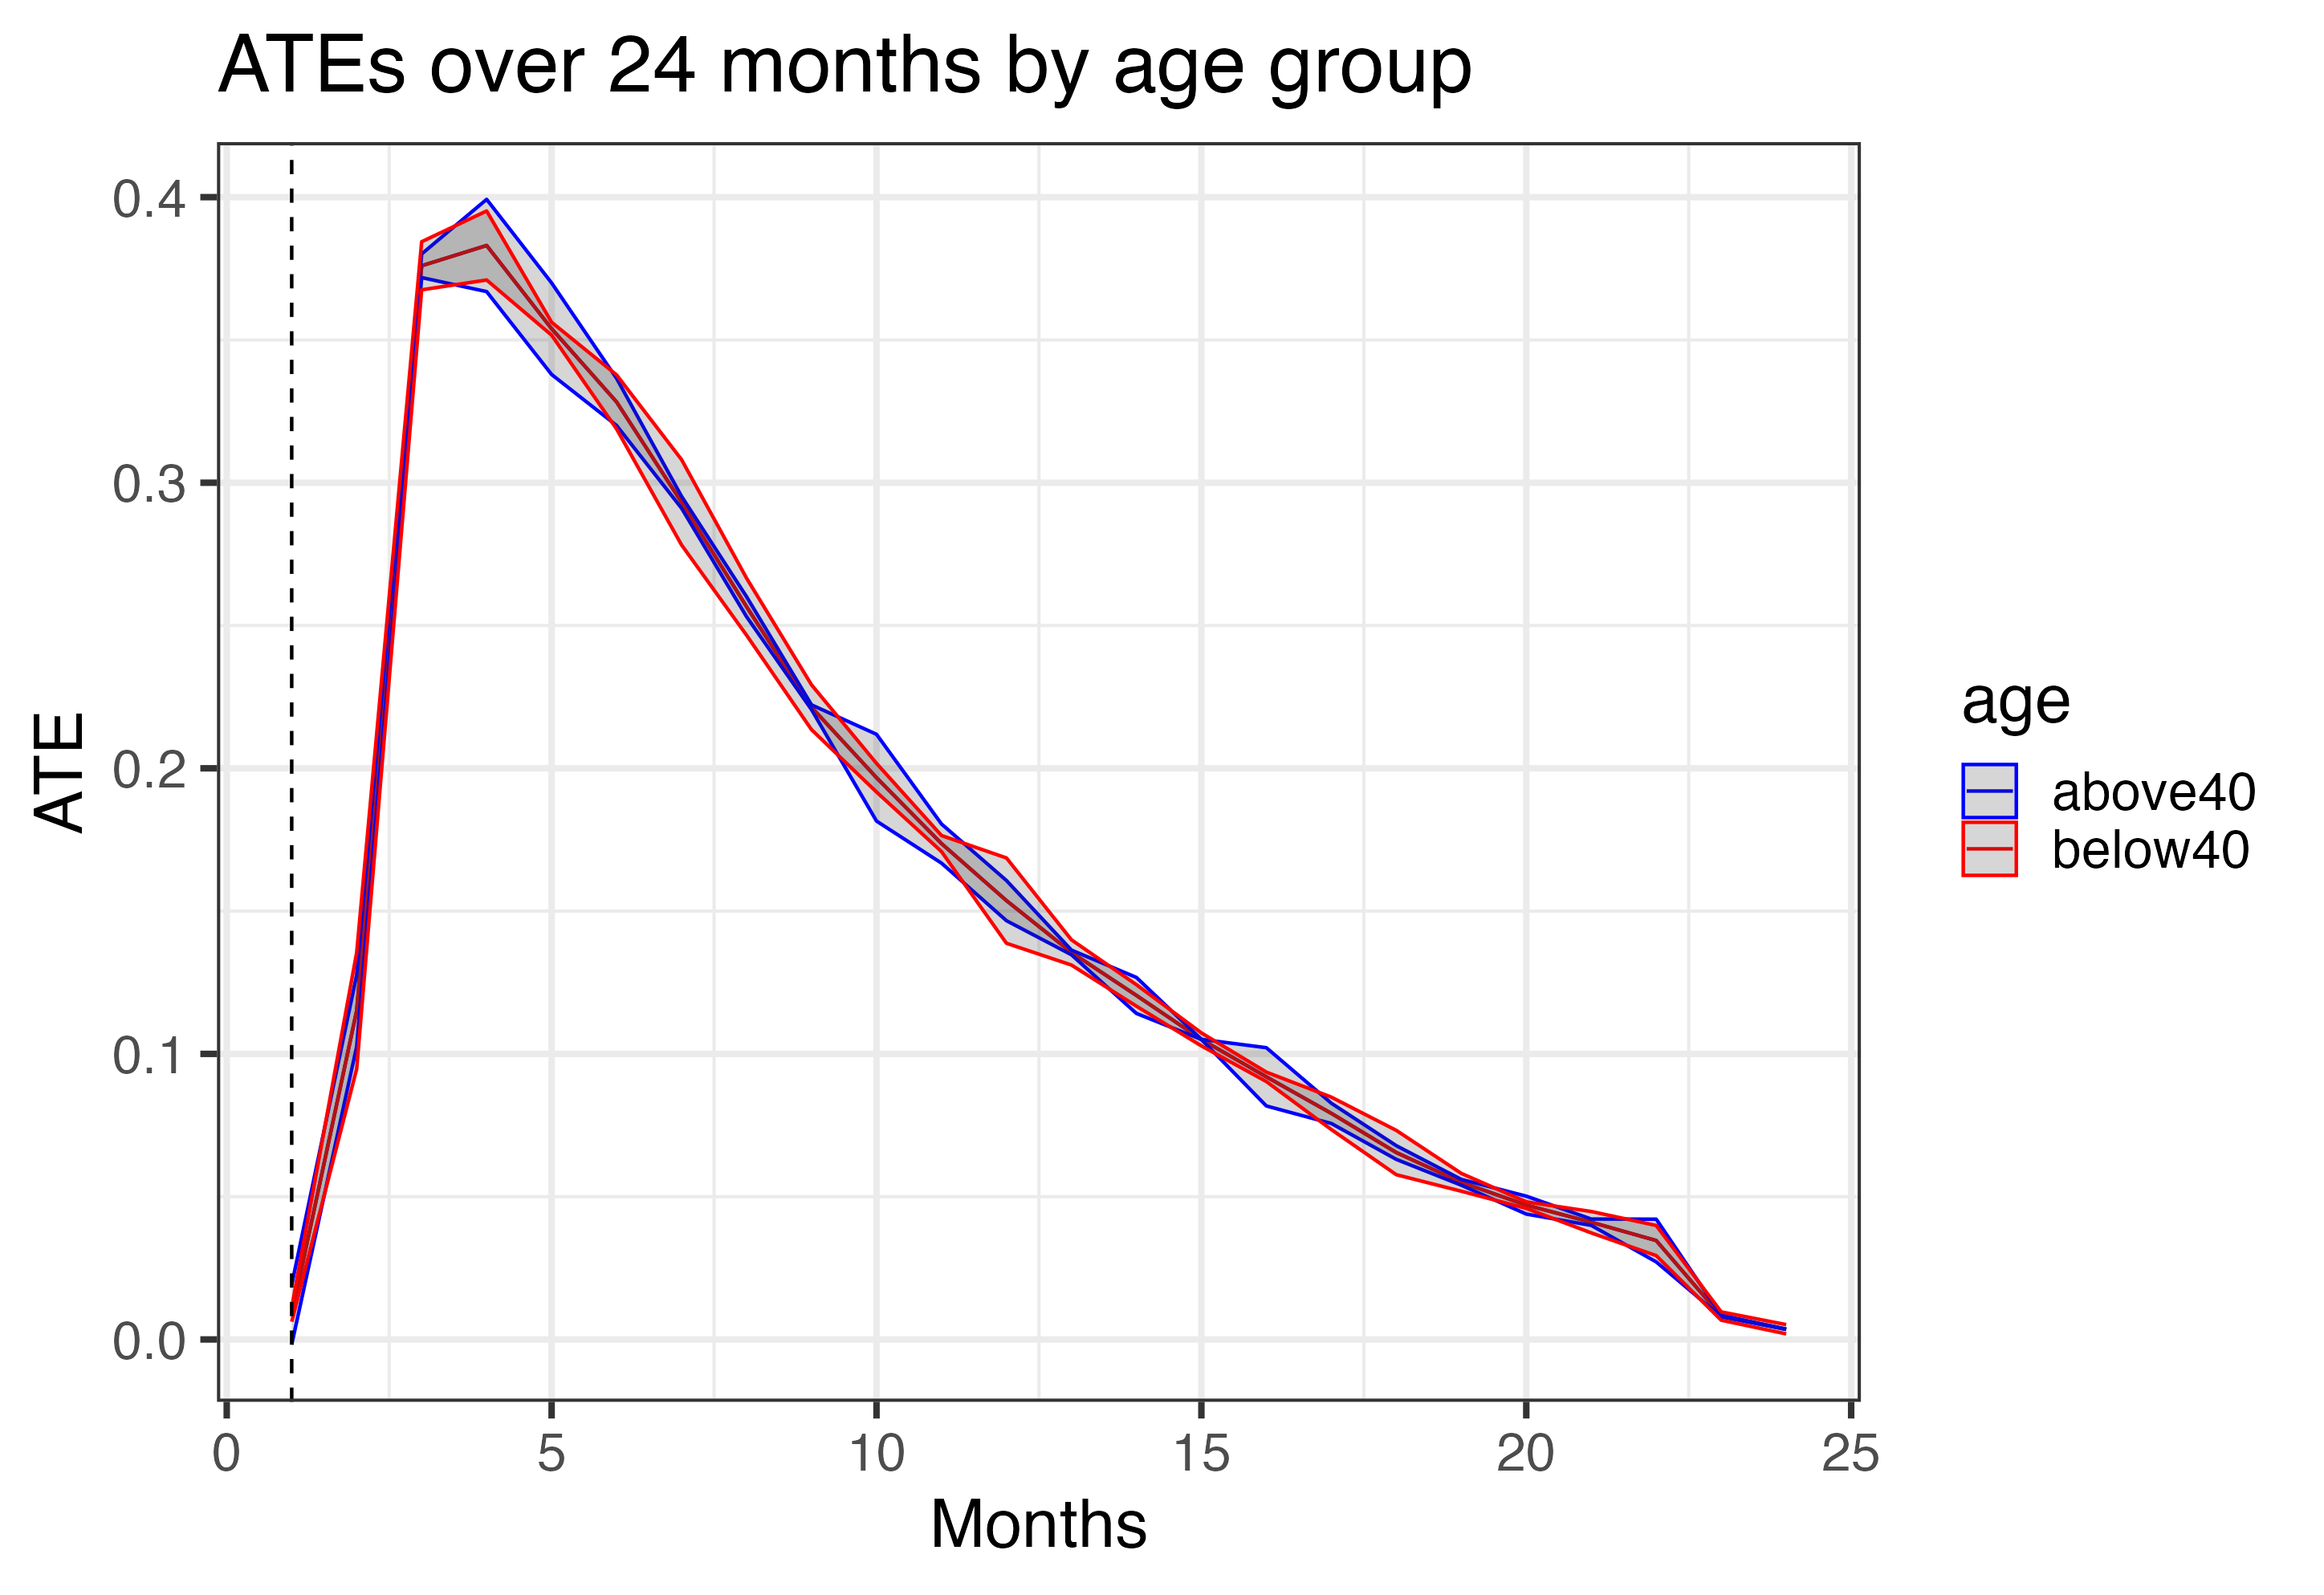
\includegraphics[width=0.7\linewidth]{ATEs_over_24_months_by_age_group.png}
    \caption{Program and Employment: ATEs over 24 months by age group}
    \label{fig:enter-label}
\end{figure}

The ATET describes the treatment effect for those that end up treated. Here, treatment assignment is not random and there may be selection into treatment. We use propensity score matching to calculate a valid counterfactual given the covariates of the entire sample assuming we observe all confounders. By pivoting from the ATE to ATET we would be estimating a counterfactual for the treated alone. If the treatment group differs from the non-treated in their potential outcome, they are not the same.

\section*{Question 4}

\subsection*{(a) Discuss potential bias from labor market competition}

The control group would have lower employment than the true counterfactual. The estimated effect would be larger that it actually is. 

\subsection*{(b) Identify assumption being violated}

The bias arises from a violation of A1, the stable unit treatment value assumption. SUTVA defines our outcome as a function of our treatment status and potential outcomes alone. The treatment received by the treated group should not impact the outcome of the non-treated group.

\subsection*{(c) Think of reverse bias scenario}

If treatment impacted the outcomes of the control group in the other direction, it can decrease the bias coming from the SUTVA violation explained in (a). An example would be if participant success raised overall demand for labor. Then non-participants’ outcomes might improve when others are treated. If the size of this bias is the same as the initial SUTVA violation explained in (a), it would fully counter this bias.

\section*{Question 5}

%The treatment group is defined as the locations $j$ in the 10km x 10km grid cell that are connected to the backbone network and are in countries that will be connected to at least one submarine cable. Therefore, the control group is defined as those locations $j$ that are not connected to the backbone network. \\

\marco{The treatment group includes all locations that gain access to fast Internet in a given quarter or year. Specifically, these are locations situated within 500 meters of the national backbone network at the time when that backbone becomes connected to at least one submarine Internet cable. \\
The control group, by contrast, consists of locations that are farther than 500 meters from the backbone network and therefore are not directly exposed to fast Internet when the submarine cable arrives.} \\

The post-treatment period starts at time period $t$ at which country $c$'s backbone network is connected to at least one submarine cable. The pre-treatment period is thus the time period before the network has been connected. \\

It is important to note that the comparison is within countries, meaning that the control groups only include non-connected locations in the same country where some locations did receive the treatment.   

\section*{Question 6}

\subsection*{(a) Why not individual fixed effects?}



The data is in repeated cross-sections, so the survey that are distributed in the same location in different time periods might have a different composition. Therefore, the authors control for any fixed differences between connected and unconnected parts of each grid-cell, which helps address potential selection bias in the placement of the backbone infrastructure. 

%There is an issue if people with higher potential employment outcomes self-select (migrate) into cells with access to the backbone.

\subsection*{(b) Why not location-specific time fixed effects?}

The treatment variable varies at the location level, so including location-specific time period fixed effects would absorb all the time-varying shocks at the location level, and thus absorb the variation that allows them to estimate the treatment effect.

\end{document}
